\documentclass[doublespacing]{report} [12px]%,doublespacing
\usepackage{graphicx}
\usepackage{tocbibind}
\usepackage{hyperref}
\usepackage{amsmath}
\usepackage{graphicx}
\usepackage{array}
\usepackage{booktabs}
\usepackage{geometry}
\usepackage{float}
\usepackage{amsfonts}
\usepackage{lmodern}
\usepackage{setspace}
\usepackage{geometry}
\begin{document}

\pagenumbering{gobble} % No page numbers 
\begin{titlepage}
\centering
   % \vspace{0.2cm}
    \Large\textbf{KWAME NKRUMAH UNIVERSITY OF SCIENCE AND TECHNOLOGY}
    
    %\Huge\textbf{(KNUST)}
    %\vspace{0.2cm}
      %\vspace{0.2cm}
  % \large{DEPARTMENT OF STATISTICS AND ACTUARIAL SCIENCE}
    %\vspace{0.2cm}
    
     \begin{center}

\includegraphics[width=0.5\textwidth]{logo.png}\end{center}

    \large{\textbf{Decoding Student Retention and Churn of
Vodafone (Telecel) in Kwame Nkrumah University
of Science and Technology (KNUST)}}
%\vspace{0.2cm}
   \\
   %\large{\textbf{A Survival Analysis Approach}}
    \vspace{0.3cm}
    
\large{Musah Faridu Oubda

Kassim Asana

Sarpong Linda

Torsi Edmond Collins

Asiamah Ezekiel}

    \vspace{0.2cm}  
    \small{A THESIS SUBMITTED TO THE DEPARTMENT OF STATISTICS AND ACTUARIAL SCIENCE, KWAME NKRUMAH UNIVERSITY OF SCIENCE AND TECHNOLOGY IN FULFILLMENT OF THE REQUIREMENT FOR THE AWARD OF THE DEGREE OF BACHELOR OF SCIENCE IN ACTUARIAL SCIENCE}\\
    \vspace{0.2cm}
    {August 20,2024}


\end{titlepage}

% Start numbering with Roman numerals for the Declaration
\pagenumbering{roman}
\chapter*{Declaration}

\vspace{1cm}

We, therefore, affirm that this paper is entirely our own original work and has not been submitted in whole or in part for another degree award in any other university. Due credit has also been given to previously published works and online publications through referencing. 
\vspace{2cm}

\begin{tabbing}
    \hspace{6cm} \= \hspace{4cm} \= \hspace{5cm} \kill
    \textbf{Musah Faridu Oubda} \> \makebox[4cm]{\dotfill} \> \makebox[4cm]{\dotfill} \\
    \textit{Student (4325620)} \> \textit{Signature} \> \textit{Date} \\[1.5cm]
    \textbf{Kassim Asana} \> \makebox[3cm]{\dotfill} \> \makebox[3cm]{\dotfill} \\
    \textit{Student (4323020)} \> \textit{Signature} \> \textit{Date} \\[1.5cm]
    \textbf{Sarpong Linda} \> \makebox[3cm]{\dotfill} \> \makebox[3cm]{\dotfill} \\
    \textit{Student (4330720)} \> \textit{Signature} \> \textit{Date} \\[1.5cm]
    \textbf{Torsi Edmond Collins} \> \makebox[3cm]{\dotfill} \> \makebox[3cm]{\dotfill} \\
    \textit{Student (4331420)} \> \textit{Signature} \> \textit{Date} \\[1.5cm]
    \textbf{Asiamah Ezekiel} \> \makebox[3cm]{\dotfill} \> \makebox[3cm]{\dotfill} \\
    \textit{Student (4316720)} \> \textit{Signature} \> \textit{Date} \\[1.5cm]
\end{tabbing}
This thesis has been submitted and we as university supervisors affirm our approval of
its submission.\\


\begin{tabbing}
 \hspace{6cm} \= \hspace{4cm} \= \hspace{5cm} \kill
     \textbf{Certified by:}\\ 
    \textbf{Miss Sandra Addai-Henne} \> \makebox[3cm]{\dotfill} \> \makebox[3cm]{\dotfill} \\
    \textit{Supervisor} \> \textit{Signature} \> \textit{Date} \\[1.5cm]
    \textbf{Certified by:}\\ 
\textbf{Prof. Gabriel Asare Okyere } \> \makebox[3cm]{\dotfill} \> \makebox[3cm]{\dotfill} \\
    \textit{Head of Department} \> \textit{Signature} \> \textit{Date}
\end{tabbing}


\newpage
\chapter*{Dedication}

We dedicate this project to the Almighty God, who has seen us through all of our challenges during this thesis period and has brought us this far. We also dedicate this effort to our families and friends, who have been there for us every step of the way with love and prayers. Finally, we dedicate this presentation to our supervisor, who stood by us through it all.  

\newpage
\chapter*{Acknowledgement}

We are grateful to the Great and Mighty God for giving us the ability and fortitude to do this task. Our sincere gratitude also extends to Miss Sandra Addai-Henne, our supervisor, who acted as a beacon of hope for us as we set out on our path. We will always remember her kindness, comprehension, and level of tolerance. She always mentored and corrected us. We also want to express our gratitude to all of the instructors at Kwame Nkrumah University of Science and Technology(KNUST) who assisted us with our studies. We are grateful to you everyone.  


\newpage
\tableofcontents

\newpage
\listoffigures

\newpage
\listoftables



 
\newpage
\chapter*{Abstract}



\newpage
\chapter{Introduction}

% Start numbering from here
\pagenumbering{arabic}

\section{Background of Study}

Ghana's telecommunications industry has experienced significant growth in recent years, with companies such as Vodafone playing a crucial role in providing mobile and internet services to people across the country \cite{bandim2022}. The industry is highly competitive, making customer retention vital for sustaining market share and profitability. Obtaining new customers is more expensive than retaining existing ones due to marketing activities, incentives, and campaigns involved. Therefore, retaining a customer is preferable to acquiring a new one. Customer churn, also known as customer attrition, refers to the loss of subscribers or customers who cease using a company’s service or product within a given period \cite{Koranchirath2024}. Understanding the reasons behind customer churn helps to develop strategies to improve customer retention and help reduce churn rates in the long run.

Vodafone is one of the leading national telecommunications providers in Ghana. As of January 2020, it had over 9.3 million mobile voice subscribers, representing 13.81\% of Ghana's market share. Since becoming the majority shareholder, Vodafone Ghana has been operating the Ghana Satellite Earth Station (GSES) since 2008 \cite{vodafone_ghana}. GSES allows Ghana to access and utilize communications satellites orbiting the Earth for various applications, such as telephone services, internet connectivity, television broadcasting, data transmission, disaster management, and emergency communications. The operation of the earth station by Vodafone Ghana proves the company's commitment to investing in and upgrading Ghana's satellite communications capabilities.
%citation for this part
In 2016, Vodafone partnered with Kwame Nkrumah University of Science and Technology (KNUST) to provide enhanced packages of services to the various faculties across the university's campuses to improve education services \cite{vodafone_knust}. This collaboration included telecommunications services such as SIM cards and data plans for the student and employee communities.

In February 2023, Telecel acquired 70\% shares in Vodafone, rebranding the company name to Telecel in 2024 \cite{telecel_ghana}. This rebranding aimed to improve service offerings across voice and data services, money transfers, and business solutions. Telecel, founded in 1986, is an Africa-focused telecommunication company that operates primarily in Africa and converges telecommunications with fintech, e-commerce, and tech startups.

%citation for this part

Student churn is a major issue every telecom company encounters. It leads to a loss of revenue and increases the cost of acquiring new customers. In the highly competitive telecom market, where customers have multiple service provider options, retaining customers becomes even more challenging. Companies use modern technology, computer software, and survival analysis approaches to identify at-risk students and devise strategies to enhance retention rates. This method of recognizing unsatisfied customers is known as churn prediction.

On March 14, 2024, Vodafone, along with several other telecommunications companies, was hit by outages on several underwater fiber optic cables, leading to disruptions in services, particularly internet services \cite{ghanaweb2023}. It affected about 10 countries in West Africa, including Ghana. Initially, it was estimated that the problem would be fixed within 3 days; however, this was not the case. The damage was massive, affecting the West Coast route to Europe, West Africa Cable System (WACS), and the Africa Coast to Europe (ACE), resulting in MainOne and SAT3 going offline \cite{apnews2023}. The only network that was properly functioning at the moment in Ghana was AirtelTigo (AT). To quickly prevent the loss of valuable customers to AirtelTigo, Vodafone (Telecel) took the initiative to update its customers daily on their progress and offer various bonuses to prevent customers from defecting to their competitors. This continued until the problem was fixed on April 29, 2024, when the WACS cable was repaired.

Previous studies have explored various factors that influence customer churn in a telecommunications company. This study aims to focus on the KNUST student population, uncover and analyze data gathered from students, apply survival analysis models to identify patterns related to churn (such as demographics, usage patterns, etc.), develop retention strategies, evaluate the success of these efforts, and make informed decisions.

\section{Problem Statement}

Regardless of efforts made by KNUST to partner with Telecel to provide affordable and accessible mobile communications services to the university’s populace, churn still persists. There is a lack of understanding about the factors driving student churn and retention, making it difficult to develop effective strategies to address this issue \cite{kapur2018}. This research aims to investigate the factors contributing to student churn and develop a survival analysis model for detecting at-risk students and design specific strategies to improve retention rates. It also seeks to enhance Telecel’s services, improve student experience, and foster long-term relationships between Vodafone (Telecel) and KNUST.

\section{Research Objectives}

The study aims to use survival analysis to estimate student churn rates at various levels. In addition, the paper aims to estimate which covariates affect the churn rate.
%\subsection{Main Objective}
%\begin{itemize}
    %\item 
%	To develop a survival analysis techniques model to detect at-risk students to improve student retention and reduce churn of Telecel at KNUST.
%	%\end{itemize}
%	
%	\subsection{Specific Objectives}
%	\begin{itemize}
%	    \item Exploring the factors that influence student churn and retention.
%	    \item Using survival analysis models to identify students at risk of churning.
%	    \item Analyzing time-to-event data to understand the patterns and timing of student churn.
%	    \item Identifying strategies to improve retention rates and reduce churn.
%	\end{itemize}

%\section{Research Questions}
%\begin{itemize}
%    \item What factors influence student retention and churn for Telecel services at KNUST?
%    \item What is the relationship between student demographics (age, gender, year of study) and churn behavior?
%    \item How does the churn rate vary with different Telecel services (voice service, data service, internet service)?
%    \item How does the quality of Telecel network and services (coverage, internet speed) influence student retention and churn?
%    \item How can Telecel services be optimized to better meet the needs and preferences of KNUST students?
%\end{itemize}

\section{Significance of the Study}

The study offers a comprehensive understanding of the factors impacting student churn from Vodafone. This will enable the development of precise strategies to enhance retention rates, thereby minimizing churn. The study will empower KNUST to improve the telecom services offered to its students. By identifying the factors influencing student retention and churn, KNUST can work closely with Telecel to guarantee the delivery of top-notch, dependable services to its students, thereby solidifying the partnership between KNUST and Telecel. The study is all about understanding what the populace expects from Vodafone (Telecel). By knowing their specific needs and preferences, the services can be improved upon. This means improved connectivity, service plans, and less hassle from switching providers. Ultimately, it ensures a more stable and reliable service for students.

\section{Structure of the Study}

The study on student retention and churn for Telecel services at KNUST aims to investigate the factors that drive students' decisions on Telecel services usage. The study follows a structured approach.
\\Chapter one discusses the background information and the foundation for the research. The problem statement and goals are stated here.
\\Chapter two of the study contains a literature review, including several studies related to the subject at hand.
\\The third chapter focuses on the methodology and data collection techniques. There are several ways of approaching this problem, but the main focus of the study is using a survival analysis modeling tool.
\\The fourth chapter presents the models and practical application to the dataset. Detailed analysis is presented here with the aid of figures and diagrams to determine the optimal model for the research.
\\Chapter five delves into the conclusion and summarizes the results obtained. Based on the findings, recommendations are formulated.

\section{Limitation of the Study}

The limitation of this research was that the data survey only included students of KNUST who were present during the annual college elections. As a result, the coverage was limited to undergraduate students on the main campus.

\newpage
\chapter{Literature Review}


\section{Introduction}
Mobile technology has become widely used, changing how students interact, communicate, and obtain information \cite{Alqatani2020}. Student retention and churn are critical issues for universities and telecom companies alike. In the context of Vodafone's services offered to students, understanding student behavior and preferences is crucial for effective retention strategies. This project addresses this gap using survival analysis, a statistical method for examining data over time \cite{BoxSteffensmeier2020}. In this context, the event of interest is student churn, defined as the discontinuation or cessation of Vodafone SIM cards. By applying survival analysis, this project will provide valuable insights into student retention and churn factors.

\subsection{Telecommunication Industry and Customer Behavior}
The telecommunication industry is highly competitive, with customer acquisition and retention being pivotal to a company's success. Research indicates that factors such as service, pricing, customer support, and competitive offerings significantly influence customer churn \cite{Lai2021}.

\subsection{Student Retention and Telecom Services}
Students, as a demographic, exhibit unique usage patterns and service expectations. Studies show that reliable connectivity, affordable pricing, and additional benefits like educational resources influence their choice of telecom services \cite{SmithBrown2020}. For telecom companies, understanding these factors is crucial to tailoring services that meet students’ needs and enhance retention.

\subsection{History of Survival Analysis (SA)}
The origins of SA and its history spread far back to the early work on mortality by John Graunt, who published the book \textit{Natural and Political Observations on the Bills of Mortality} in 1662. The concept of “Life Tables” was introduced in this book. A new, modern era in SA started during World War II in the USA, where the reliability of military equipment was tested using SA. After World War II, SA became popular and spread to various other disciplines \cite{Jerenz2008}. The most influential papers on SA were published by Kaplan and Meier \cite{Kaplan1958} and Cox \cite{Cox1972}, in which the Kaplan-Meier product limit estimator and Cox proportional hazard model were introduced, respectively.

\subsection{Application of Survival Analysis}
Survival analysis (SA) has been successfully applied in diverse fields, including medical research, engineering (reliability analysis), finance, and economics. In finance, SA has been used to analyze a firm's vulnerability to global financial crises and identify firms at risk of failure, enabling timely interventions \cite{Lee2014, Pereira2014, Kumar2015, Iwasaki2014}. SA has also been employed to predict the optimal time to buy or sell stocks within the stock market \cite{Kumar2015}. In the banking sector, SA is utilized to assess banks' survival during financial crises, measure their strength when entering new markets \cite{Leung2010, Evrensel2008}, and conduct credit risk analysis \cite{Tsujitani2012, Baesens2005}. The widespread adoption of SA across these domains underscores its versatility and effectiveness in modeling time-to-event data and identifying the factors that influence outcomes of interest.

\section{Conceptual Review}

\subsubsection{Customer Retention and Churn}
Customer retention refers to a company's capacity or ability to maintain or retain their customer base over a specific period. High retention rates are crucial for maintaining revenue streams, reducing marketing costs associated with acquiring new customers, and fostering a positive brand reputation. Customer churn, also known as customer attrition, is the rate at which customers stop using a company's product or service \cite{Masarifoglu2019} . It can be caused by various factors such as dissatisfaction with the service, better offers from competitors, or changes in personal circumstances. In the telecommunications industry, market competitiveness is measured by churn rate. Telephone, internet, and mobile services are all part of telecommunications.

\section{Empirical Studies}
%Include reference in the bibliography
Imani, M. (2020). \textit{Customer Churn Prediction in Telecommunication Using Machine Learning: A Comparison Study}. This paper tackles customer churn in telecoms, emphasizing that retaining customers is cheaper than acquiring new ones. It evaluates various machine learning methods for predicting churn by comparing classifiers, target detectors, feature extraction, and feature selection techniques. The study finds that Random Forest and Feed-Forward Neural Networks with Genetic Algorithm showed high accuracy. Effective target detectors included Spectral wngle Mapper and Adaptive Subspace Detector. Clustering-Based Feature Extraction and Advanced Binary Ant Colony Optimization excelled in improving classification and feature selection. The study recommends implementing Random Forest and Neural Networks for effective churn prediction.

Melik Masarifoglu and Ali Hakan Buyuklu (2019). \textit{Applying Survival Analysis to Telecom Churn Data}. This paper emphasizes the importance of customer retention in telecoms, noting that retaining customers is more cost-effective than acquiring new ones. It employs survival analysis to estimate customer survival and hazard functions, focusing on factors like campaigns, tariffs, tenure, age, and auto-payment. The paper introduces survival analysis (SA) as a statistical method to analyze time-to-event data. It describes the Cox Proportional Hazard Model (CPHM), a widely used technique for quantifying the risk of an event occurring during the observation period. The paper uses Kaplan-Meier estimates and the Cox model to analyze the impact of various predictors on customer churn. The results show how different factors, such as campaigns and tariffs, affect customer survival probabilities. The study finds that survival analysis is effective for predicting churn and recommends its use for targeting at-risk customers and improving retention strategies.

Sitti Nurhaliza et al (2022). \textit{A comparison of cox proportional}
The research paper conducts a comparative analysis of the Cox Proportional Hazard (CPH) model and Random Survival Forest (RSF) to evaluate their effectiveness in survival analysis. The CPH model, a well-established method, is known for its interpretability, allowing researchers to understand the relationship between covariates and survival time. However, it assumes proportional hazards, which may not hold in all cases. In contrast, RSF is a non-parametric ensemble method that can handle complex, non-linear relationships and does not require the proportional hazards assumption. The study uses data from various domains, such as medicine and engineering, to assess the performance of both models. The findings suggest that while RSF generally offers better predictive accuracy, especially in cases with non-linear relationships, CPH remains valuable for its simplicity and interpretability. The paper concludes that the choice between CPH and RSF should be based on the specific requirements of the analysis, balancing the need for interpretability against predictive accuracy.




\newpage
\chapter{Methodology}

\section{Introduction}

This chapter structures the research methods and procedures followed by the analysis to predict student churn of Vodafone (Telecel) in KNUST. A comprehensive explanation of the research models, mathematical formulations and interpretations are presented here. The paper compares their performance using the Concordance Index thus shedding light on their predictive capabilities.

\section{Research Design}

The study employs quantitative research. This type of research aims to establish the cause-and-effect relationships between variables. Specifically, it focuses on quantifying various aspects of students’ usage and satisfaction, rather than exploring underlying meanings or personal experiences in an open-ended manner.

\section{Pilot Survey}

Before the actual statistics were carried out, a pilot survey was held to grasp the scope of students’ understanding of the topic. It was carried out using final year students in Actuarial Science. Out of 50 questionnaires sent out, a total of 46 respondents were returned. 

\section{Data Collection}

The primary data source for this research was a survey conducted among students at Kwame Nkrumah University of Science and Technology (KNUST) in College of Science. The survey targeted students in final years (Level 400). The dataset includes a variety of questions, each capturing specific aspects relevant to the study with the aid of Google Forms.


\section{Sample Size}
The sample size of the research was determined through simple random sampling. Simple random sampling is a sampling technique in which each member of the population has an equal chance of being selected. This method ensures that the sample is representative of the population, as every individual has an equal probability of being included. This sampling technique is employed to determine the optimal sample size as it is a straightforward method that allows for unbiased estimation of the population parameters.

The sample size for simple random sampling can be determined using the formula below:

\begin{equation}
n_0=\frac{z^2 \ast p \ast \left(1-p\right)}{E^2}
\end{equation}
\begin{equation}
n=\frac{n_0}{1+(\frac{n_0-1}{N})}
\end{equation}

Where:
\begin{itemize}
    \item \((N)\) is the population size.
    \item \((n_0)\) is the initial sample size for simple random sampling.
    \item \((n)\) is the adjusted sample size for the population.
    \item \((z)\) represents the critical value.
    \item \((p)\) is the estimated proportion of the population
    \item \((E)\) is the margin of error.
\end{itemize}

Parameter Justification:

\begin{itemize}
    \item \textbf{Z-score} \((z)\): A confidence level of 95\% is chosen, resulting in a Z-score of 1.96.
    \item \textbf{Population} \((N)\): The population size of the College of Science students is about 2,835.
    \item \textbf{Estimated Proportion} \((p)\): To maximize sample size, we use 0.5.
    \item \textbf{Margin of Error} \((E)\): 5\% since the confidence level is 95\%.
\end{itemize}

\begin{equation}
n_0 = \frac{\left(1.96^2 \times 0.5 \times 0.5\right)}{0.05^2}
\end{equation}
\begin{equation}
n_0 \approx 383.82
\end{equation}
\begin{equation}
n_0 \approx 384
\end{equation}
\begin{equation}
n = \frac{384}{1 + \left(\frac{384 - 1}{2835}\right)}
\end{equation}
\begin{equation}
n \approx 338.297
\end{equation}
\begin{equation}
n \approx 338
\end{equation}

A simple random sample size of 354 students from the population of about 2,835.


\section{Data Pre-Processing}

In the realm of data analysis, ensuring the quality and suitability of data is paramount for deriving meaningful insights and making informed decisions. The initial phase of the study involved a thorough examination of the dataset to identify and handle missing data appropriately to ensure that subsequent analyses were conducted on a complete and representative dataset. One of the critical preprocessing tasks involved the transformation of categorical variables into numeric format. This was achieved using label encoding, a technique that assigns unique integer labels to each category with the aid of Python. The transformation restructured the dataset to facilitate survival analysis. The data was then organized to facilitate essential components such as time duration, event indicators, and relevant covariates to the variables. 
The lifelines package played a pivotal role in this section by providing essential survival analysis models in Python. The models are crucial for analyzing data where the time to student churn is important. 

\section{Concept of Survival Analysis}

Survival analysis is a branch of statistics used to analyze time-to-event data. The primary interest lies in the time until the occurrence of the event of interest.  The time variable is usually referred to as survival time since it gives the time that an individual has survived over some follow-up period. The event is also referred to as a failure because the event of interest is usually death, disease incidence, or some other negative experience. 

\section{Censoring}

In survival analysis, not all subjects may experience the event of interest within the study period. Censoring occurs when the survival time of a subject is not fully observed. It occurs when a subject leaves the study before an event occurs, or when the study ends before the event has occurred for all subjects.


\subsection{Right-Censored}

It occurs when a subject has some loss to follow up or the study ends before the event of interest occurs. The lifetime is known to exceed a certain value meaning that, true survival time is equal to or greater than the observed survival time.

\subsection{Left-Censored}

It occurs when the event of interest has occurred before the study starts, and thus the exact survival time is known only to be less than a certain value indicating that the true survival time is less than or equal to the observed survival time.

\subsection{Interval-Censored}

It can occur if a subject’s true but unobserved survival time is within a certain known specified time interval. Interval-censoring incorporates both right-censoring and left-censoring. 

\begin{figure}[H]
    \centering
    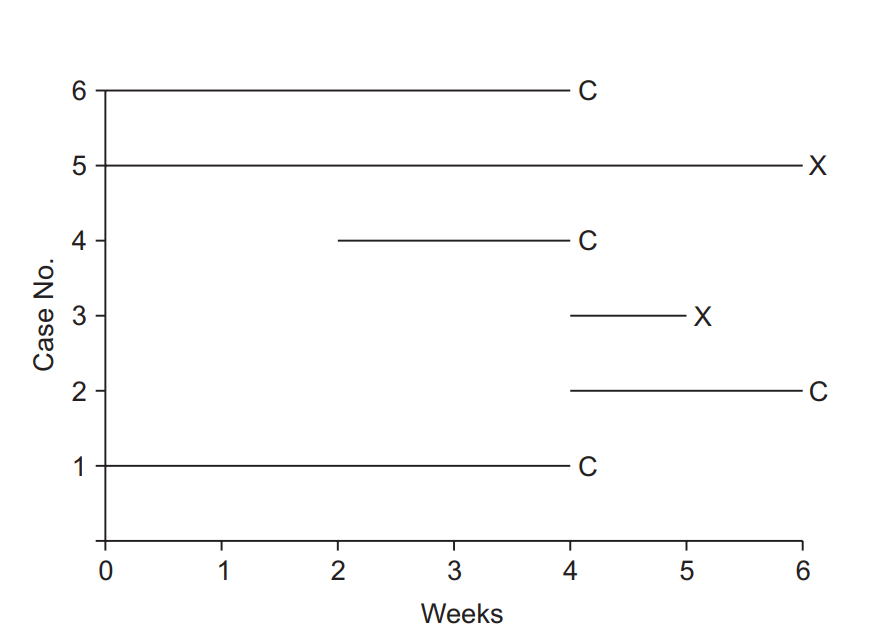
\includegraphics[width=0.5\linewidth]{Figure 3/3.2.png}
    \caption{Censoring Graph}
    \label{Figure 3.2}
\end{figure}


\begin{itemize}

\item \(C\) indicates censored data
\item  \(X\) indicates observed events


\end{itemize}



\section{Fundamental Concepts of Survival Analysis}

\subsection{\texorpdfstring{Survival Function \( S(t) \)}{Survival Function S(t)}}
The survival function \(S\left(t\right) \) also known as the survival probability function, gives the probability that a person survives longer than some specified time.  Let \(T\) be a non-negative continuous random variable representing the elapsed time until an event occurs. The probability density function (pdf) of \(T\) is denoted by \(f(t)\), and the cumulative distribution function (cdf) is denoted by \(F(t)\). The cdf \(F(t)\) is defined as:
\begin{equation}
F(t) = \Pr\{T < t\}
\end{equation}
The survival function \(S(t)\) is the complement of the cummulative distribution function and is given by:
\begin{equation}
S(t) = 1 - F(t)
\end{equation}
\begin{equation}
S(t) = \Pr\{T \geq t\}
\end{equation}
\begin{equation}
S(t) = \int_t^\infty f(u) \, du
\end{equation}
The derivative of \(S(t)\) with respect to \(t\) is:
\begin{equation}
S'(t) = -F'(t)
\end{equation}
\begin{equation}
S'(t) = -f(t)
\end{equation}
In figure \ref{Figure 3.3} below, the curve on the left is a theoretical curve of the survival function\ \(S\left(t\right) \) which ranges from 0 up to infinity. It is non-increasing and therefore slopes downward as \(t\) increases. At \(t= 0\), \(S\left(0\right)=1\) and when \( t\ =\ \infty , S\left(\infty\right)\ =\ 0.\) 
When actual data is used, the survivor curve does not result in a smooth curve but rather obtains a step function graph. The step function is illustrated on the right in \ref{Figure 3.3}.  The study period is never infinite in duration as there may be competing risks for failure, it is possible that not everyone obtains the event of interest. The estimated survivor function \(\hat{S}\left(t\right)\), thus may not go all the way down to 0 at the end of the study.

\begin{figure}[H]
    \centering
    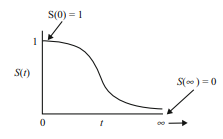
\includegraphics[width=0.45\textwidth]{Figure 3/3.31.png}
    \hfill
    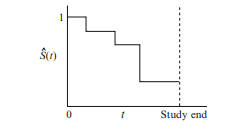
\includegraphics[width=0.45\textwidth]{Figure 3/3.32.png}
    \caption{Survivor Curves}
    \label{Figure 3.3}
\end{figure}

\subsection{\texorpdfstring{Hazard Function \( h(t) \)}{Hazard Function h(t)}}

The hazard function \( h(t)\ \)denotes the instantaneous rate of failure at time \(t\), given that the subject has survived up to time\( (t).\)

\begin{equation}
h(t) = \lim_{\Delta t \to 0} \frac{P(t \le T < t + \Delta t \mid T \geq t)}{\Delta t}
\end{equation}
\begin{equation}
h\left(t\right)\geq0
\end{equation}


The hazard function \( h\left(t\right)\), is given by the formula: \(h\left(t\right)\ \)equals the limit, as \(\Delta t \) approaches zero, of a probability statement about survival, divided by \(\Delta t\), where \(\Delta t\) denotes a small interval of time.

\begin{align}
h(t) &= \lim_{\Delta t \to 0} \frac{\Pr(t \leq T < t + \Delta t \mid T > t)}{\Delta t} \\
&= \lim_{\Delta t \to 0} \left[ \frac{\Pr(t \leq T < t + \Delta t)}{\Delta t} \cdot \frac{\Delta t}{\Pr(T > t)} \right] \\
&= \lim_{\Delta t \to 0} \left[ \frac{\Pr(t \leq T < t + \Delta t)}{\Delta t} \right] \cdot \lim_{\Delta t \to 0} \left[ \frac{1}{\Pr(T > t)} \right] \\
&= \frac{1}{S(t)} \cdot \lim_{\Delta t \to 0} \left[ \frac{\Pr(t \leq T < t + \Delta t)}{\Delta t} \right] \\
&= \frac{1}{S(t)} \cdot \lim_{\Delta t \to 0} \left[ \frac{F(t + \Delta t) - F(t)}{\Delta t} \right] \\
&= \frac{f(t)}{S(t)} \\
\end{align}

The hazard function is also known as the conditional failure rate. It is a rate rather than a probability. In the hazard function formula, the expression to the right of the limit sign gives the ratio of two quantities. The numerator is a conditional probability while the denominator, \(\Delta t\) denotes a small-time interval. By the division, a probability per unit of time is obtained, which is no longer a probability but a rate. In particular, the scale for this ratio is not 0 to 1 like a probability but rather ranges between 0 and infinity while depending on whether time is measured in days, weeks, months, or years. 

\begin{equation}
H(t)=\int_{0}^{t}{h(x)dx}
\end{equation}

The cumulative hazard function \(H(t)\) can be derived from the hazard function. It is the integral of the hazard function up to time \(t\). It represents the total hazard experienced up to time \( t. H(t)\) provides a straightforward cumulative measure of risk or failure over time.

\begin{equation}
S(t) = \exp\left[-\int_{0}^{t} h(x) \, dx\right]
\label{eq:survival_function}
\end{equation}

\begin{equation}
h(t) = -\left[\frac{dS(t)/dt}{S(t)}\right]
\end{equation}

The equations above clearly defines the relation between the hazard function and survival function. This can be seen in (3.25) and (3.26) in which the $h(t)$ gives the $S(t)$ and vice versa.


\section{Approaches in Survival Analysis}

The approaches to use in survival analysis are underlined by their strengths and weaknesses. The choice is based on statistical assumptions, data characteristics and the complexity of the survival patterns to model.

\subsection{Parametric Methods}

These methods assume that the survival times follow a specific statistical distribution. Common parametric survival models are exponential, Weibull, log-normal and gamma models. They estimate parameters using maximum likelihood estimation or Bayesian methods.

\subsection{Non-Parametric Methods}

These methods include approaches that make minimal assumptions about the form of the survival distribution. Common non-parametric methods in survival analysis are the Kaplan-Meier Estimator, Nelson-Aalen Estimator and Log-Rank Test.

\subsection{Semi-Parametric Methods}

Semi-parametric models combine parametric elements (the effect of covariates) with non-parametric elements (the baseline hazard function) such as the Cox Proportional Hazard.

\section{Kaplan Meier}
The Kaplan-Meier estimator is employed in survival analysis to analyze the time until an event occurs. The Kaplan-Meier estimator calculates the survival probability at a specific time step by multiplying the probability of surviving each previous time step.
The estimator is computed as
\begin{equation}
S\left(t\right)=\prod_{i:t_i\le t}\left(1-\frac{d_i}{n_i}\right)
\end{equation}
Where:
 \begin{itemize}
     \item \(t\) is a time
     \item \(d_i \) the number of events (churn) at time \(t_i\)
     \item \(S\left(t\right)\ \)is the survival probability at time \(t\)
     \item \(n_i\) is the number of individuals at risk just before time \(t_i\)
 \end{itemize}
The estimator essentially calculates the probability of surviving from one time step to the next, and the product of these probabilities gives the overall survival probability up to time \(t\).

\section{Cox Proportional (Cox PH) Hazard Model}

The Cox Proportional Hazards model is a popular semi-parametric model to check the relationship between the survival time and a set of predictors.

\begin{equation}
h\left(t \mid x\right) = h_0(t) \exp(\beta_1 x_1 + \beta_2 x_2 + \cdots + \beta_p x_p)
\end{equation}

Where:
 \begin{itemize}
     \item \(h(t\mid x)\) is the hazard function, i.e., the instantaneous rate of the event occurring at time \(t\) given the predictor variables \(x\).
     \item \(h_0\left(t\right)\) is the baseline hazard function, representing the hazard for individuals with all predictor variables equal to zero.
     \item \(\beta_1,\beta_2,\ldots,\beta_p\) are the coefficients for the predictor variables
 \end{itemize}

 The coefficients \(\beta\) are estimated using maximum likelihood estimation, and the model assumes a proportional hazard ratio, meaning the effect of the predictors on the hazard is constant over time.
An important assumption on the Cox PH is that it has a constant hazard function proportion for each time. The Hypothesis of the assumption is as follows: 
                 \begin{equation}
\begin{array}{c}
H_0: \text{The Assumption of Proportional Hazard is fulfilled} \\
H_1: \text{The Assumption of Proportional Hazard is not fulfilled}
\end{array}
\end{equation}
with rejection test $H_0$ if the $p-value < 0.05$.

\section{Accelerated Failure Time (AFT)}

In situations where the Cox proportional hazards assumption is not satisfied, the parametric model approach can be used. Accelerated Failure Time (AFT) is one of the popular parametric models used in survival analysis. The model assumes that the survival function \(S(t)\) follows a parametric continuous distribution. This implies that the distribution is following a Weibull, lognormal, or log-logistic distribution. An AFT model aims to account for the influence of multiple covariates on the survival time by either accelerating or decelerating it.

\begin{equation}
\lambda(x) = \exp(b_0 + \sum_{i=1}^{n}{b_i x_i})
\end{equation}
Where:
\begin{itemize}
    \item \(\lambda(x)\) is the accelerating factor
    \item \(b_0\) is the baseline accelerating factor when all covariates are 0
    \item \(b_i\) is the regression coefficient for the \(i\)-th covariate
    \item \(x_i\) are the covariates
\end{itemize}


\subsection{Weibull AFT}
The Weibull distribution is flexible and can model increasing or decreasing hazard rates, making it suitable for a wide range of survival data.

\begin{equation}
    S(t) = \exp\left(-\left(\frac{t}{\lambda}\right)^\gamma\right)
\end{equation}

where \(\lambda\) is the scale parameter and \(\gamma\) is the shape parameter.

\subsection{Lognormal AFT}
Assumes that the logarithm of the survival time follows a normal distribution. It's suitable for data where the event time is skewed to the right.

\begin{equation}
    S(t) = 1 - \Phi\left(\frac{\log(t) - \mu}{\sigma}\right)
\end{equation}

where \(\mu = b_0 + \sum_{i=1}^{n}{b_i x_i}\) is the location parameter, \(\sigma\) is the scale parameter, and \(\Phi\) is the cumulative distribution function of the standard normal distribution.

\subsection{Log-logistic AFT}
 Assumes that the logarithm of the survival time follows a logistic distribution. It can handle both increasing and decreasing hazard rates, similar to the Weibull model.

\begin{equation}
    S(t) = \left(1 + \left(\frac{t}{\lambda}\right)^\gamma\right)^{-1}
\end{equation}

where \(\lambda\) is the scale parameter and \(\gamma\) is the shape parameter.


 
\section{Information Criteria}

Information criteria are used to evaluate and compare the relative quality of statistical models. They help in model selection by balancing model fit with complexity, penalizing models that use more parameters to avoid overfitting. The three most commonly used criteria are the Akaike Information Criterion (AIC), Bayesian Information Criterion (BIC), and Hannan-Quinn Criterion.

\subsection{Akaike Information Criterion (AIC)}

The Akaike Information Criterion (AIC) is a widely used measure that balances the goodness of fit of the model with the number of parameters. A lower AIC indicates a better model fit.

\begin{equation}
AIC = 2k - 2\ln(L),
\end{equation}

Where:
\begin{itemize}
    \item \(k\) is the number of parameters in the model.
    \item \(L\) is the likelihood of the model.
\end{itemize}

\subsection{Bayesian Information Criterion (BIC)}

The Bayesian Information Criterion (BIC) is another criterion for model selection, similar to AIC but with a stronger penalty for the number of parameters. This makes BIC more conservative when choosing models.

\begin{equation}
BIC = k\ln(n) - 2\ln(L),
\end{equation}

Where:
\begin{itemize}
    \item \(k\) is the number of parameters in the model.
    \item \(n\) is the number of observations in the dataset.
    \item \(L\) is the likelihood of the model.
\end{itemize}

\subsection{Hannan-Quinn Criterion (HQ)}

The Hannan-Quinn Criterion (HQ) is used less frequently than AIC and BIC but provides another option for model selection. HQ lies between AIC and BIC in terms of penalization strength.

\begin{equation}
HQ = 2k\ln(\ln(n)) - 2\ln(L),
\end{equation}

Where:
\begin{itemize}
    \item \(k\) is the number of parameters in the model.
    \item \(n\) is the number of observations in the dataset.
    \item \(L\) is the likelihood of the model.
\end{itemize}


\section{Concordance Index in Survival Analysis}

The Concordance Index, often referred to as the C-index or Harrell's C-index, is a statistical metric used to evaluate the performance of models in survival analysis. It assesses how well a model discriminates between subjects in terms of their event times and predicted risks. 

The Concordance Index measures the model's ability to correctly rank the predicted risks of individuals based on their actual event times. The Concordance Index evaluates whether the model's predicted risks align with the observed event times.

\begin{equation}
C=\frac{Number\ of\ Concordant\ Pairs}{Number\ of\ Concordant\ Pairs\ +Number\ of\ Discordant\ Pairs}
\end{equation}

A \(C\) value above 0.5 suggests that the model has predictive ability better than random chance. A higher \(C\) value implies a better model performance and more accurate risk predictions.



\newpage
\chapter{Analysis and Findings}
\section{Introduction}

This section presents the study's findings and discusses what each output means towards the research goals. It includes easy-to-read tables, graphs, and computer results based on the methods used. The analysis closely examines details towards the model building, diagnostics and evaluation. The information here was obtained from using python for computer analysis during the research. This chapter seeks to explain the use of survival models in the methodology to determine the Vodafone (Telecel) churn rate among students.

\section{Data Description}

The dataset has a shape consisting of 338 rows and 14 columns from a sample of students in KNUST's College of Science. The Churn covariate is assigned as the event while the Churn\_Level is assigned as the time to the event (duration). The remaining covariates are used to explain the event and duration.

\begin{table}[H]
    \centering
    \begin{tabular}{ll}
        \toprule
        \textbf{Variable}& \textbf{Description} \\
        \midrule
        Gender & Gender of the student\\
        Churn & Whether the student has churned\\
        Residence & Place of residence in school\\
        Usage Frequency & Frequency of vodafone sim usage\\
        Voice Calls & Usage of voice calls \\
        Mobile Data Internet & Usage of mobile data/internet \\
        SMS Text Messaging & Usage of SMS/text messaging \\
        Data Exhaustion & Whether monthly data allowance (5GB) is exhausted\\
        Multiple Networks & Use of other networks \\
        Poor Network Quality Coverage & Perception of poor network quality/coverage \\
        Unsatisfactory Customer Service & Perception of unsatisfactory customer service \\
        High Costs Pricing & Perception of high costs/pricing \\
        Monthly Data Usage & Monthly Data Usage\\
        Churn Level & Level at which the student churn\\
        \bottomrule
    \end{tabular}
    \caption{Description of Variables}
    \label{tab: 4.1}
\end{table}



\section{Descriptive Analysis}
\begin{table}[H]
\centering
\begin{tabular}{cccc}
\hline
\textbf{Variable} & \textbf{Unique} & \textbf{Mode}& \textbf{Frequency} \\
\hline
Gender & 2 & Female & 233 \\
Churn & 2 & No & 320 \\
Residence & 2 & Off-campus & 280 \\
Usage Frequency & 5 & Daily & 157 \\
Voice Calls & 2 & Yes & 272 \\
Mobile Data Internet & 2 & Yes & 295 \\
SMS Text Messaging & 2 & Yes & 183 \\
Data Exhaustion & 2 & Yes & 280 \\
Multiple Networks & 2 & Yes & 301 \\
Poor Network Quality Coverage & 2 & Yes & 241 \\
Unsatisfactory Customer Service & 2 & No & 216 \\
High Costs Pricing & 2 & Yes & 190 \\
Monthly Data Usage & 5 & 8 and more & 239 \\
\hline
\end{tabular}
\caption{Summary Statistics of Categorical Variables}
\label{table:summary_statistics}
\end{table}



\subsection{Kaplan Meier (KM) Curve}

The Kaplan-Meier survival curve below is a tool to estimate the probability that students will remain enrolled in the study over a given time period. 
\begin{figure}[H]
    \centering
    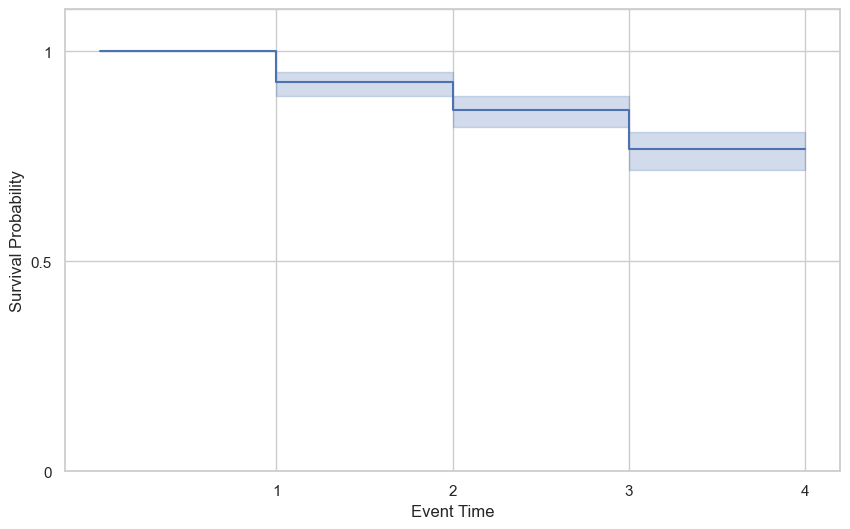
\includegraphics[width=1\linewidth]{Figure 4/4.1.png}
    \caption{Kaplan Meier Curve}
\end{figure}

The x-axis represents the event time. The 0 indicates when the study began whiles 4 represents when the study ends. The y-axis represents survival probability and ranges from 0 to 1. Each step down indicates an event, which decreases the overall survival probability.  The shaded area around the line suggests the confidence interval, giving a range within which the true survival curve is expected to lie.

In churn prediction, this curve helps identify critical time points where student retention drops significantly and allows institutions to intervene proactively. 



\subsection{Kaplan Meier Analysis}

The provided Kaplan-Meier estimator output in Table 4.2 below summarizes the survival curve in Table 4.1 over the levels in KNUST.


\begin{table}[H]
\centering
\begin{tabular}{cccccc}
\toprule
Event Time & Number of Individuals & Number of Events & Survival Probability & Lower CI & Upper CI \\
\midrule
0 & 338 & 0 & 1.000000 & 1.000000 & 1.000000 \\
1 & 338 & 25 & 0.926036 & 0.892497 & 0.949406 \\
2 & 313 & 22 & 0.860947 & 0.819283 & 0.893630 \\
3 & 291 & 32 & 0.766272 & 0.717405 & 0.807836 \\
4 & 259 & 0 & 0.766272 & 0.717405 & 0.807836 \\
\bottomrule
\end{tabular}
    \caption{Kaplan-Meier Survival Analysis Results}
    \label{tab:km_results}
\end{table}


Initially, at time 0 in \ref{tab:km_results} (when students initially start the academic year), all 338 students are considered to be at risk. With no events (churns) recorded yet, the survival probability is 1.
As the students ascend the academic ladder, the number at risk begins to gradually decrease as some begin to experience the event. The higher the number of events, the more the number at risk decreases. 
At the end of the first year, 25 students experienced the event of interest and therefore are omitted from the study at the beginning of the second year.  Anytime the event of interest is experienced, they are omitted from the study until the study duration ends.   
The confidence intervals (Lower Cl and Upper CI) provide ranges within which the true survival probabilities lie with a certain level of confidence.


\section{Cox Proportional Hazard (COX PH)}

In the Cox Proportional Hazard modeling, two things are mostly done, namely, partial testing for each predictor variable and testing the Cox Proportional Hazard assumption. 
 
Furthermore, the results of parameter estimation and partial testing are presented in the Table below.

% Insert another Table

\begin{table}[H]
\centering
\begin{tabular}{lccc}
\toprule
Variable & Coefficient ($\beta$) & Standard Error & P-value\\
\midrule
Gender & 0.33 & 0.28 & 0.24 \\
Residence & 0.32 & 0.27 & 0.25 \\
Usage Frequency & -0.08 & 0.07 & 0.27 \\
Voice Calls & -0.57 & 0.32 & 0.08 \\
Mobile Data Internet & 0.32 & 0.46 & 0.48 \\
SMS Text Messaging & 0.48 & 0.25 & 0.06 \\
Data Exhaustion & -0.20 & 0.38 & 0.61 \\
Multiple Networks & -0.13 & 0.44 & 0.78 \\
Poor Network Quality Coverage & 2.60 & 0.35 & <0.005 \\
Unsatisfactory Customer Service & -1.40 & 0.30 & <0.005 \\
High Costs Pricing & -1.13 & 0.29 & <0.005 \\
Monthly Data Usage & 0.21 & 0.09 & 0.02 \\
\bottomrule
\end{tabular}
\caption{Cox Proportional Hazards Model Results}
\label{tab:cox_ph_results}
\end{table}


The coefficient columns in \ref{tab:cox_ph_results} provides information about the relationship between each independent variable and the dependent variable. A positive coefficient indicates an increase in the independent variable is associated with an increase in the hazard (risk) of churn (event). A higher value of these variables is associated with a higher likelihood of churn occurring. 

Conversely, a negative coefficient suggests a decrease in the hazard (risk) of churn (event). A higher value of these variables is associated with a lower likelihood of churn occurring.

The p-value column helps assess the statistical significance of each independent variable. A low p-value (typically  \(<\) 0.05) indicates that the covariate is likely to have a meaningful impact on the event. This can be seen in Monthly Data Usage, Poor Network Quality Coverage and High Costs Pricing.

\begin{figure}{H}
    \centering
    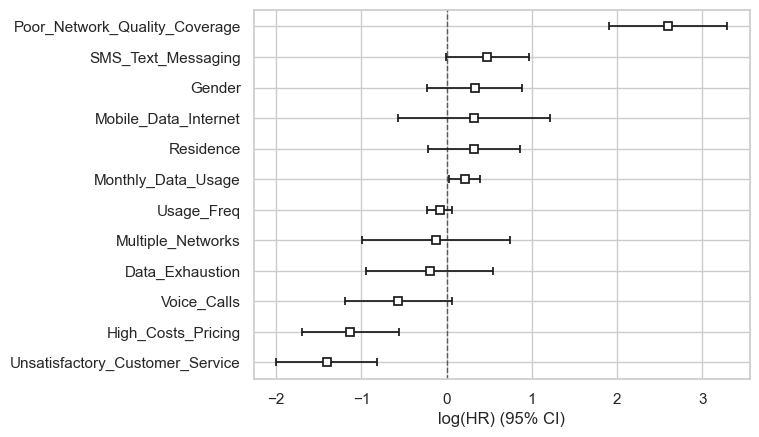
\includegraphics[width=1\linewidth]{Figure 4/4.2.png}
    \caption{Cox PH Forest Plot}
    \label{cox ph forest}
\end{figure}

\ref{cox ph forest} above is a forest plot of the Cox PH. A coefficient to the right of zero (positive log hazard ratio) indicates that an increase in that variable is associated with a higher risk of a student churning. A coefficient to the left of zero (negative log hazard ratio) indicates that an increase in that covariate is associated with a lower risk of a student churning.
The further a coefficient is from zero, the stronger the effect of that covariate on the hazard of churn.
The horizontal lines extending from the boxes are the 95\% confidence intervals, showing the uncertainty around these estimates. If the confidence interval crosses zero, the covariate is not statistically significant.

\subsection{Cox PH Assumption Test}
This test checks if the impact of the predictor variables on the hazard rate is constant over time. Covariates violating this assumption might need further investigation or transformation.	

The null hypothesis states that there is a significant relationship between the predictor variables (such as College and Voice Calls) and the likelihood of a student churning.

The alternative hypothesis suggests that there is no significant association between the predictor variables and the likelihood of churn.


\begin{table}[H]
\centering

\begin{tabular}{lcc}
\toprule
Covariate& Test Statistic & p-value \\
\midrule
Data Exhaustion & 0.46 & 0.50 \\
Gender & 0.26 & 0.61 \\
High Costs Pricing & 1.74 & 0.19 \\
Mobile Data Internet & 0.63 & 0.43 \\
Monthly Data Usage & 1.49 & 0.22 \\
Multiple Networks & 0.09 & 0.77 \\
Poor Network Quality Coverage & 2.36 & 0.12 \\
Residence & 0.01 & 0.93 \\
SMS Text Messaging & 0.04 & 0.84 \\
Unsatisfactory Customer Service & 0.10 & 0.76 \\
Usage Frequency & 0.04 & 0.84 \\
Voice Calls & 2.70 & 0.10 \\
\bottomrule
\end{tabular}
\caption{Test statistics of Cox-PH Assumption Test}
\label{tab:test_statistics}
\end{table}


The Cox Proportional Hazard method has a weakness in that the proportional hazard assumption must be met. In \ref{tab:test_statistics}, it can be seen that most covariates meet the assumptions as their p-values are above 0.05 meaning that there is no strong evidence against the proportional hazard’s assumption for these covariates.

This means that the assumption of the hazard ratios are constant over time holds for all the covariates.



\section{Accelerated Failure Time (AFT) }

The Accelerated Failure Time (AFT) model is a possible alternative that can be used when the Cox Proportional Hazard (PH) model does not hold. The study uses the AFT in order to understand the direct effect of covariates on survival time.

\begin{table}[H]
    \centering
    \begin{tabular}{lccc}
        \hline
        Model & AIC & BIC & Hanna-Quinn \\
        \hline
        WeibullAFTFitter & 316.433303  & 300.079395& 306.67379\\
        \textbf{LogNormalAFTFitter}& \textbf{305.805320}& \textbf{289.451411}& \textbf{306.67379}\\
        LogLogisticAFTFitter & 307.510343& 291.156435& 306.67379\\
        \hline
    \end{tabular}
    \caption{Comparison of AIC, BIC, and Hanna-Quinn values for different AFT models}
    \label{tab:model_comparison}
\end{table}


\noindent
\textbf{Results:} \\
The AFT model with the lowest AIC is: \textit{LogNormalAFTFitter} \\
The AFT model with the lowest BIC is: \textit{LogNormalAFTFitter} \\
The AFT model with the lowest Hanna-Quinn is: \textit{WeibullAFTFitter}

The study compares three Accelerated Failure Time (AFT) models—Weibull, Log-Normal, and Log-Logistic—using AIC, BIC, and Hanna-Quinn criteria in \ref{tab:model_comparison}. The results reveal that the Log-Normal AFTFitter consistently has the lowest AIC and BIC, indicating a better overall fit despite the Weibull AFTFitter achieving the lowest Hanna-Quinn value.

\subsection{Log-Normal Model}
% Table here


\begin{table}[H]
\centering
\begin{tabular}{lccc}
\toprule
Variable & Coefficient ($\hat{\beta}$) & Standard Error (SE) & P-value\\
\midrule
Data Exhaustion& 0.102 & 0.148 & 0.493 \\
Gender & 0.032 & 0.118 & 0.785 \\
High Costs Pricing & 0.515 & 0.122 & <0.0005 \\
Mobile Data Internet & -0.287 & 0.207 & 0.165 \\
Monthly Data Usage & -0.069 & 0.044 & 0.113 \\
Multiple Networks & -0.104 & 0.202 & 0.607 \\
Poor Network Quality Coverage & -1.041 & 0.123 & <0.0005 \\
Residence & -0.146 & 0.124 & 0.239 \\
SMS Text Messaging & -0.228 & 0.108 & 0.036 \\
Unsatisfactory Customer Service & 0.809 & 0.122 & <0.0005 \\
Usage Frequency & -0.002 & 0.033 & 0.940 \\
Voice Calls & 0.132 & 0.135 & 0.329 \\
Intercept (for $\mu$) & 1.626 & 0.393 & <0.0005 \\
Intercept (for $\sigma$) & -0.616 & 0.084 & <0.0005 \\
\bottomrule
\end{tabular}
\caption{Lognormal Model Coefficients}
\label{table:lognormal_coefficients}
\end{table}

Unlike the Cox PH analysis, the coefficient columns in \ref{table:lognormal_coefficients} provide information about the relationship between the covariates to event time (Churn\_Level). A positive coefficient indicates a decrease in the time it takes to the event. A negative coefficient suggests an increase in the time to the event. 

 A higher value of these covariates is associated with a higher  likelihood of the time to the event occurring if positive and lower chance of occurring if negative.
 
The p-value column helps assess the statistical significance of each covariate. A low p-value (typically  \(< \) 0.05) indicates that the covariate is likely to have a meaningful impact on Churn\_Level. 

The mu\_intercept is the mean baseline when the covariates are 0 and the sigma\_intercept is the standard deviation used to estimate the variance to determine the spread when the covariates are 0.

\begin{figure}[H]
    \centering
    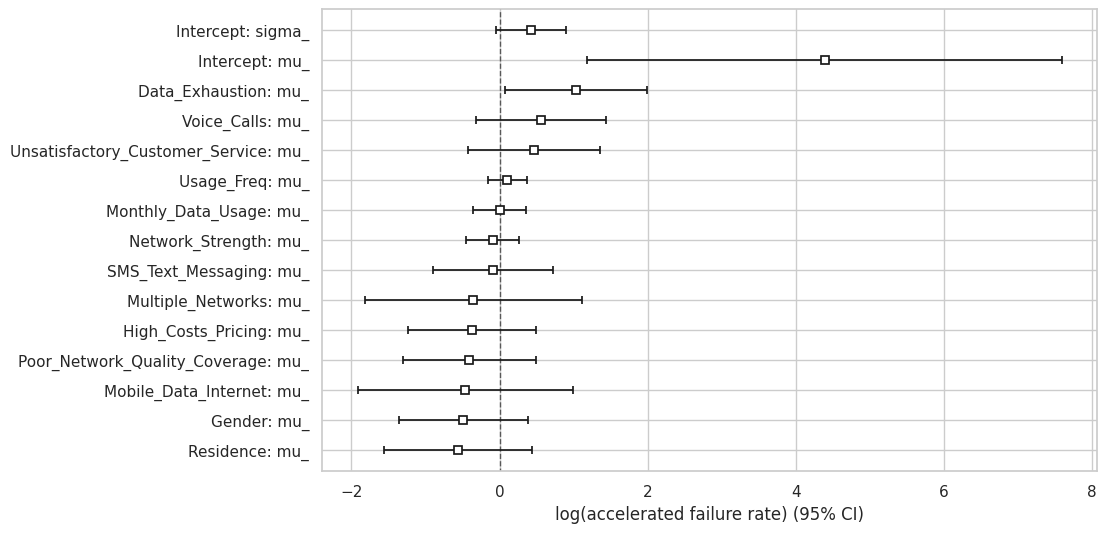
\includegraphics[width=0.8\linewidth]{Figure 4/4.4.png}
    \caption{LogNormal Forest Plot}
    \label{LogNormal}
\end{figure}

The boxes (squares) in the plot represent the estimated coefficients for each factor in the Lognormal AFT model in \ref{LogNormal}. The positive values suggest that the covariate decrease the time to the event, while negative values suggest it increases the time to the event. The horizontal lines extending from the boxes are the 95\% confidence intervals, showing the uncertainty around these estimates. If the confidence interval crosses zero, the covariate is not statistically significant.

\section{Model Comparison}

In this section, the models used are compared based on the AIC and the concordance values. The higher the concordance, the better the model predictive value and the smaller the AIC, the better the model fit.

%Table here
	\begin{table}[H]
			\centering
			\begin{tabular}{lcc}
				\toprule
				\textbf{Model} & \textbf{Concordance} & \textbf{Loglike hood}\\
				\midrule
				LogNormal& 0.958& 	290.678\\
				Cox PH & 0.96& 	266.68\\
				\bottomrule
			\end{tabular}
			\caption{Model Concordance and AIC values}
			\label{Table 2}
			
		\end{table}

Based on the comparison of the concordance values and log-likelihood in Table \ref{Table 2}, it is evident that the Cox PH model shows a higher concordance compared to the LogNormal model, indicating a better predictive value. However, the log-likelihood values suggest that the LogNormal model has a better fit. 

\newpage
\chapter{Conclusion}


\bibliographystyle{apalike}
\bibliography{references.bib}


\end{document}
 